\documentclass[11pt]{amsart}
\usepackage{geometry}                % See geometry.pdf to learn the layout options. There are lots.
\geometry{letterpaper}                   % ... or a4paper or a5paper or ... 
%\geometry{landscape}                % Activate for for rotated page geometry
%\usepackage[parfill]{parskip}    % Activate to begin paragraphs with an empty line rather than an indent
\usepackage{graphicx}
\usepackage{amssymb}
\usepackage{epstopdf}

%\usepackage{hyperref}
\usepackage[colorlinks = true,
            linkcolor = blue,
            urlcolor  = blue,
            citecolor = blue,
            anchorcolor = blue]{hyperref}


\usepackage[ruled,vlined]{algorithm2e}

\hypersetup{
    colorlinks=true,
    linkcolor=blue,
    filecolor=magenta,      
    urlcolor=cyan,
}
 
\urlstyle{same}
\DeclareGraphicsRule{.tif}{png}{.png}{`convert #1 `dirname #1`/`basename #1 .tif`.png}


\title{Latent Channel Networks}
\author{Clifford Anderson-Bergman}

\newcommand{\edge}{e}
\newcommand{\latentedge}{\tilde e}
\newcommand{\latcon}[3]{c_{#1#2#3} }
\newcommand{\hubProb}{\theta}
\newcommand{\expEdge}{\epsilon}
\newcommand{\expCon}{C}

\begin{document}
\maketitle

\section{Abstract}

Latent Euclidean embedding models a given network by representing each node in a Euclidean 
space, where the probability of two nodes sharing an edge is a function of the distances between the nodes. 
This implies that for two nodes to share an edge with high probability, they must be relatively close in 
\emph{all} dimensions. This constraint may be overly restrictive for describing modern networks, in which having similarities 
in \emph{at least} one area may be sufficient for having a high edge probability. We introduce a new model, which we call 
Latent Channel Networks, which allows for such features of a network. We present an EM algorithm for fitting the model, 
for which the computational complexity is linear in the number of edges and number of channels
and apply the algorithm to both synthetic and classic network datasets. 

\section{Introduction}

In this work, we define a graph $G = (N, E)$, where $N$ is a set of nodes and 
$E$ is an adjacency matrix, such that $E_{ij} = 1$ if nodes $i$ and $j$ share an 
edge and $E_{ij} = 0$ otherwise. At this time, we discuss undirected graphs, implying $E_{ij} = E_{ji}$
and ignore self loops, implying $E_{ii} = 0$.
The degree of a node is defined as the number of edges attached to it. 
One classic example of this include social networks, in which nodes represent 
individuals and two individuals are considered to share an edge if they are listed as friends.
Another common example is co-authorship graphs, in which nodes represent researchers 
and they are considered to share an edge if they have coauthored a paper together. 

In the analysis of graph data, a common goal is to describe a network in a reduced order 
space, thereby providing insight of an underlying graph structure to the analyst. 
One of the simplest structures is the stochastic block model \cite{sbm}. 
In this model, each node belongs to an unobserved block, where nodes
have a fixed probability of having an edge with nodes within their block ($p_{in}$)
and another fixed probability of having an edge with nodes outside their block ($p_{out}$). 
Typically, $p_{in} >> p_{out}$ so nodes are much more likely to 
share an edge with nodes within the same block, and each block can be considered a cluster. 
Recent work  covers efficient estimation of the parameters of stochastic block models
\cite{sbmExact}, \cite{sbmSpec}, statistical characteristics of the estimators \cite{specConsist}, \cite{sbmAsym}
and model selection \cite{sbmSelection} and hierarchical stochastic block models \cite{nestedsbm}.

One disadvantage to stochastic block models is they imply that within each block, 
the expected degree of a node is constant, with a variance implied by a binomial distribution. 
This fails to capture a very commonly observed phenomenon in social networks,
namely that often a small number of nodes express an extremely high degree relative to most other nodes. 
In order to capture this, many other models have been proposed, such as the degree-corrected stochastic 
block model \cite{dcsbm}, in which edge probabilities is based on block membership
 \emph{and} a given node's degree. 

Another limitation of the stochastic block mode is that it is \emph{hard clustering} approach. 
That is to say, each node deterministically belongs to a single block, and only one block. 
Several alternatives have been considered that allow for \emph{soft clustering}. 
This includes the mixture stochastic block model \cite{msbm}, where each node belongs to a each block 
with a given probability. Another approach to tackle this problem 
by maximizing the modularity score \cite{modularity}, but with community membership 
described as a probability vector rather than a categorical variable \cite{softmod1}, \cite{softmod2}, \cite{softmod3}.
In addition to modularity, other metrics such as overlapping correlation coefficient \cite{occ} may be used. 
We note that with the exception of \cite{msbm}, these methods are 
poised as purely optimization based clustering, rather 
a probability based model.

An alternative approach that ultimately motivated this work is that of 
a latent embedding. In a Euclidean embedding model \cite{eucEmbed}, 
each node is represented in a latent Euclidean space, 
with edge probabilities being inversely proportional to distance.
Because edge probabilities are directly modeled, one can naturally 
allow edge probabilities to be a function of both latent distance
\emph{and} linear predictors associated with each node. 
This model naturally allows for both very high and very low degree
nodes; these are simply nodes whose intercept are exceptionally high or low. 
Traditional MCMC approaches are used for inference in \cite{eucEmbed}, 
although method to accelerate this include using variational Bayes \cite{vbEuc}
and stratified case-control sampling \cite{stratEuc}.
A similar approach is that of a random dot product graph \cite{randDot1}, \cite{randDot2},
in which nodes a represented in a latent space and edge probabilties
between two nodes are given by the dot product of their latent positionings. 
Estimates of the latent positions can be estimated via eigendecompositions of
the adjacency matrix \cite{eigenDot}. Clusters are not explicitly 
modeled in latent space embedding, but clustering may be performed 
on the lower-dimensional latent embedding. 


The work we present is largely inspired by latent space embedding. 
One major disadvantage of an Euclidean embedding is that in order for 
two nodes to have a high edge probability, they must be close in \emph{all}
dimensions. However, in modern social networks it seems reasonable 
that being similar in \emph{at least one} social dimension may be sufficient for high edge probability. 
To capture this dynamic, we present a Latent Channel Model, in which 
two nodes will share an observed edge in the graph if they are connected through 
at least one unobserved latent channel.
The probability of two nodes connecting through a given channel 
is the product of each node's frequency of use of the given channel. 
If one considers channels to represent communities, our model can be viewed 
as something similar to a soft-clustering model. 
Under this interpretation, an important distinction between our model and 
other soft-clustering approaches that we are aware of is that we do not constrain 
community membership to sum to one. 
This very naturally models networks
that contain a mix of high degree nodes (nodes that use multiple channels with high frequency)
and low degree nodes (nodes that have low frequencies associated with all channels). 

In section \ref{sec:model}, we mathematically describe our model and present various ways
to interpret meaningful parameters from the model. In section \ref{sec:algorithm}, we present 
both a simple and more complicated but more computationally efficient algorithm to compute the maximum 
likelihood estimate of the model parameters. In section \ref{sec:applications}, we apply the model 
to two stochastic block model networks and several classic real networks. 

\section{Latent Channel Model}
\label{sec:model}
\subsection{Model Parameterization}

Let use define an undirected graph $G$ with nodes $n_1$,...,$n_{N_n}$ and edges $\edge_{ij} = 1$ if $n_i$ and $n_j$ are connected and 0 otherwise. 
Define $N_n$ to be the number of nodes and $N_e$ to be the number of edges of the graph.
We augment this observed graph with a latent set of channels $C_1$,...,$C_K$, which provide intermediate connections between nodes. 
In particular, we introduce latent edges $\latentedge_{ikj}$, which is equal to 1 if node $n_i$ shares a latent edge to channel $h_k$ toward node $n_j$.
Our model dictates that a pair of nodes share an observed edge on the graph if they are both fully connected through one or more latent channel. More formally, 

\[
\edge_{ij} = 
\begin{cases}
1 & \text{if there exists } k \text{ such that } \latentedge_{ikj} = \latentedge_{jki} = 1 \\
0 & \text{otherwise}.\\
\end{cases}
\]

This is illustrated on figures \ref{fig:unconnected} and \ref{fig:connected}. For simplicity, we define

\begin{equation}\label{eq:hubConDef}
\latcon{i}{j}{k} = \mathbb{I}( \latentedge_{ikj} = \latentedge_{jki} = 1 ).
\end{equation}

In other words, $\latcon{i}{j}{k}$ is an indicator that nodes $i$ and $j$ are connected through channel $k$. 

\begin{figure}
\centering
\begin{minipage}{0.5\textwidth}
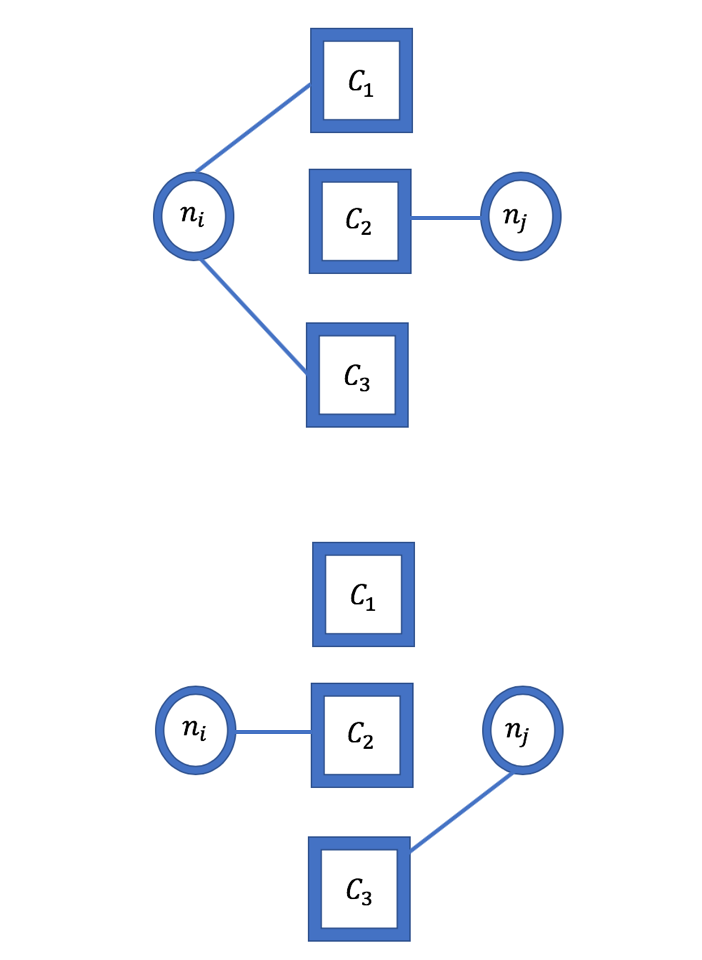
\includegraphics[width = 6cm, height = 8cm]{LatentUnconnected.png}
\caption{Nodes $n_i$ and $n_j$ do not share an edge as they are not connected through any channel.}
\label{fig:unconnected}
\end{minipage}%
\begin{minipage}{0.5\textwidth}
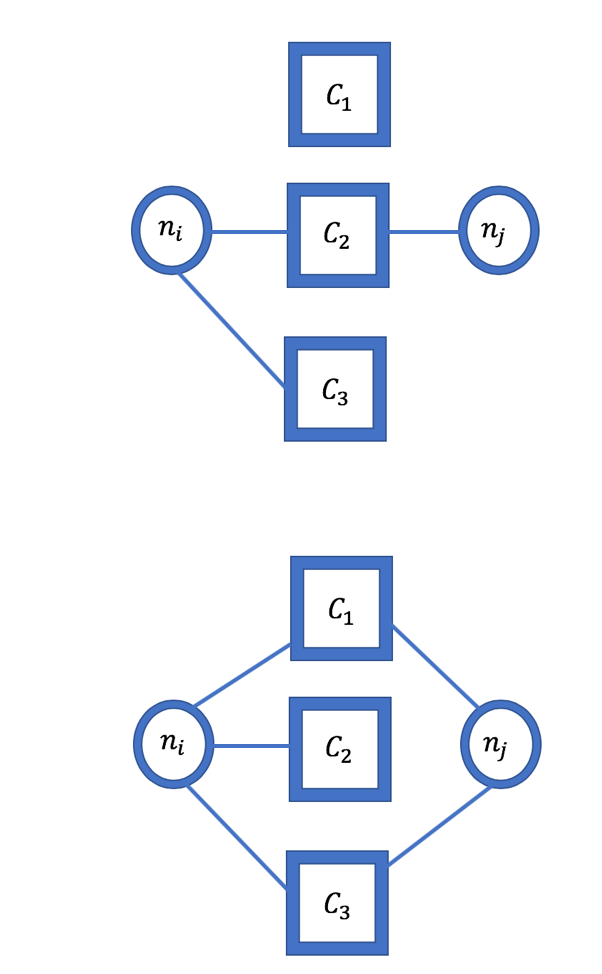
\includegraphics[width = 5cm, height = 8cm]{LatentConnected.png}
\caption{Nodes $n_i$ and $n_j$ share an edge as they are  connected through at least one channel.}
\label{fig:connected}
\end{minipage}
\end{figure}


We do not observe the $\latentedge_{ikj}$'s directly. 
However, our model dictates that for all $j$, $\latentedge_{ikj}$ are independently distributed Bernoulli 
distributions with probability $p_{ik}$. 
Thus, the marginal probability\footnote{Marginal probability meaning ignoring where $n_i$ and $n_j$ actually share an edge} 
that $n_i$ will share a edge to $n_j$ through channel $h_k$ is $p_{ik} p_{jk}$. 
To compute the probability that nodes $n_i$ and $n_j$ share an edge, we compute

\begin{equation} \label{eq:edgeProb}
\begin{split}
P(e_{ij} = 1) =   &1 - P(e_{ij} = 0) \\
			& 1 - \prod_{k = 1}^K \left(1 - P(\latentedge_{ikj} = 1 \cap \latentedge_{jki} = 1) \right) \\
                         & 1 - \prod_{k = 1}^K (1 - p_{ik} p_{jk}) \\
\end{split}
\end{equation}


In other words, the probability nodes $n_i$ and $n_j$ share an edge
is one minus the probability they do not share an edge. The probability they do not share
an edge is  the product of the probabilities they do not share an edge through any of the $K$ channels. 

As such, the log-likelihood of a latent channel graph can be written as 

\begin{equation}\label{eq:llk}
L(G | p) = \sum_{i = 2}^n \sum_{j = 1}^i 
    e_{ij} \log \left( 1 - \prod_{i = 1}^K (1 - p_{ik} p_{jk}) \right) + 
    (1 - e_{ij}) \log \left( \prod_{i = 1}^K (1 - p_{ik} p_{jk}) \right)
\end{equation}


\subsection{Interpretation of Model}


If one considers each channel to represent a latent community, then $p_{ik}$ informally represents 
the strength of node $i$'s attachment to community $k$. However, this parameter alone can be fairly hard to interpret, 
as it is unclear how large $p_{ik}$'s should be to be considered a strong connection. 
To help interpretation of the model, we present a few particularly interesting derived values. 

We first consider parameter

\begin{equation} \label{eq:condProb}
\hubProb_{ijk} = P( \latcon{i}{j}{k} = 1 | e_{ij} = 1) = \frac{p_{ik} p_{jk} } { 1 - \sum_{k = 1}^K (1 - p_{ik} p_{jk}) }.
\end{equation}

The value $\hubProb_{ijk}$ represents the probability that nodes $i$ and $j$ are connected through channel $k$, 
given that the graph contains an edge between $i$ and $j$. This is especially interesting in the case that 
channel $k$ appears to have a meaningful interpretation, such as attachment strength parameter $p_{ik}$ being correlated with meta-data
on the nodes. For example, if attachment strength to channel $k$ is strongly associated with nodes that have the occupation statistician, and 
$\hubProb_{ijk}$ is high, this suggests that given that nodes $i$ and $j$ share a connection, they have a high probability 
of having an edge through the statistical community. 
It is worth noting that 


\begin{equation}\label{eq:condProbIneq}
\sum_{k = 1}^K \hubProb_{ijk} \geq 1
\end{equation}

and typically with strict inequality. This is because two nodes that share an edge must share \emph{at least} 
one edge through a latent channel, but may share many. For example, if channel $k$ represents the statistical community 
and $k'$ represents associations through a given research institution, 
statisticians at the same institution are likely to be connected through both channels $k$ and $k'$. 

Next, we consider 

\begin{equation}\label{eq:hubsize}
S_k = \sum_{i = 1}^{N_n} p_{ik}
\end{equation}

where we refer to $S_k$ as the \emph{size} of the channel. 
One way to interpret this parameter is that if a new node $i'$ were to 
be fully connected to channel $k$, e.g. $p_{i' k} = 1$, it would be expected to have 
$S_k$ connections through channel $k$. More generally, the  expected number of connections
for a new node would be $p_{i' k} S_k$. 

Another particularly useful parameter is 

\begin{equation}\label{eq:expConnects}
\expCon_{ik} = \mathbb{E}\left[ \scriptstyle \sum_{j \neq i} \latcon{i}{j}{k} | G \right] = \displaystyle \sum_{j \neq i} e_{ij} \hubProb_{ijk}.
\end{equation}

Formula \ref{eq:expConnects} represents the expected number of connections node $i$ has through channel $k$, 
conditional on the edges observed in the graph. 
While $p_{ik}$ tells us the strength of attachment node $i$ has to 
channel $k$, it is not sufficient to determine how many connections
node $i$ has through channel $k$. For example, a strong attachment to a small channel
may result in fewer edges than a weak attachment to a large channel.
As such, this statistic can provide insight in how many connections a node has through a given 
community, which is a function of both that individual's strength of attachment to the community 
\emph{and} the size of the community. 

Similar to equation \ref{eq:condProbIneq}, we note that 

\begin{equation} \label{eq:expIneq}
\mathbb{E}\left[ \scriptstyle \sum_{j \neq i} \latcon{i}{j}{k} | G \right]  \geq \sum_{j \neq i} e_{ij}
\end{equation}

or that for subject $i$, the expected sum of connections through \emph{all} 
channels is typically greater than the sum of all observed edges in the graph associated with that node. 
Again, this is because a single edge can be the result of connections through multiple channels. 

We do suggest caution in over interpreting such parameters based on fitted data. 
As is the case for many probabilistic network models, 
we currently propose estimating the parameters via maximum likelihood estimation.
Given the high dimensional parameter space, 
standard asymptotic normality results 
should not be considered a reliable method for estimating uncertainty.
As such, we suggest using these methods for exploratory data analysis
rather than making strong inference statements about a given network. 
Alternatively, Bayesian methods could be used to determine uncertainty. 
However, to do so, one must first address the unidentifiability issue
that arises due to label switching of the channels. 

\section{Algorithm}
\label{sec:algorithm}

We differ to maximum likelihood estimation to estimate the values of $p_{ik}$. 
In general, the problem is non-identifiable, as  one can transpose the indices 
of the channels and arrive at an identical log-likelihood. Similarly, the problem is highly 
non-concave. As such, we will use an EM algorithm \cite{EM} to fit the parameters of the model. 

\subsection{Fundamental EM Algorithm}

Note that if we observed the values of $\latentedge_{ikj}$, the log-likelihood would be greatly 
simplified to 

\begin{equation} \label{eq:compllk}
L(G, \latentedge | p) = \sum_{i = 1}^{N_n} \sum_{j \neq i}^{N_n} \sum_{k = 1}^{K} \latentedge_{ikj} \log( p_{ik} ) + (1 - \latentedge_{ikj}) \log(1 - p_{ik})
\end{equation}

which has closed form solution $\hat p_{ik} = \sum_{j \neq i}^{N_n} \latentedge_{ikj}  / (N_n - 1)$, providing our M-step in the 
EM algorithm. For the E-step, we recognize that 

\begin{equation}
P(\latentedge_{ikj} = 1 | e_{ij} = 1) = 
	p_{ik} p_{jk} + p_{ik} (1 - p_{jk}) \left( 1 - \prod_{k' \neq k} ( 1 - p_{ik'} p_{jk'} ) \right)
\end{equation}

\begin{equation}
P( \latentedge_{ikj} = 1 | e_{ij} = 0) = 
	p_{ik} - p_{ik} p_{jk}
\end{equation}

We take an ECM algorithm \cite{ECM} approach, where each $p_{ik}$ is 
updated individually rather than all at once. 
This approach is particular advantageous when using caching with efficient updates.
For clarity, we first present a simple, yet computationally inefficient, 
implementation in algorithm \ref{alg:simple}. 
Noting that computing 
$P( \latentedge_{ikj} | e_{ij} = 1)$
requires $O(K)$ operations and 
$P( \latentedge_{ikj} | e_{ij} = 0)$ 
requires $O(1)$ operations,  this implementation of the algorithm requires 
$O(N_e K^2 + (N_n^2 - N_e)K)$ computations per iteration. 

\begin{algorithm}
\SetAlgoLined
\KwResult{Fixed point estimate of $N \times K$ matrix $p$}
 Adjacency Matrix $e$; K\;
 N = nrow(e)\;
 $p$ = RandomUniform(min = 0, max = 1, nrow = N, ncol = K)\;
 maxIters = 1,000; iter = 0;
 tol = $10^{-4}$; maxDiff = tol + 1\;
 \While{ iter $<$ maxIters \& tol $>$ maxDiff}{
 	pOld = p\;
	iter++\;
 	\For{ i in 1:N }{
		\For{ k in 1:K }{
			\For{ j in 1:N}{
	 			$\latentedge_{ijk} = 
				\begin{cases} 
				0 & \text{ if } i = j \\
				P( \latentedge_{ikj} | e[i,j] = 1) & \text{ else if } e[i,j] = 1 \\ 
				P( \latentedge_{ikj} | e[i,j] = 0) & \text{ otherwise} \\
				\end{cases}$
			}
			p[i,k] = $\frac{\sum_{j = 1}^N \latentedge_{ikj}}{N-1}$\;
		} 
	}
	maxDiff = max( $|$ p - pOld $|$ ) \;
 }
 \Return(p) \
\caption{Simple ECM Algorithm}
\label{alg:simple}
\end{algorithm}
 
\subsection{Efficient Caching}
 
While the algorithm described in algorithm \ref{alg:simple} is straightfoward, 
many of the computations in this algorithm are redundant and the order of complexity 
of this algorithm can be reduced by caching and updating various statistics. 

For ease of notation, we define $E_i$ to be the set of nodes that share an edge with 
node $i$ and $E_i^c $ to be the set of nodes that lack an edge with node $i$. We explicitly 
store $E_1,...,E_{N_n}$ in an edge list, but do not explicitly store $E_i^c$. Note that we define 
$i$ to be in neither $E_i$ nor $E_i^c$. 

We first note that the EM steps can be combined in the form 

\begin{equation} \label{eq:combineEM}
 p^{new}_{ik} =  \frac{ \displaystyle  \sum_{j \in E_i^c} P( \latentedge_{ikj} | e_{ij} = 0) + \sum_{j \in E_i } P( \latentedge_{ikj} | e_{ij} = 1) } {N - 1}.
\end{equation}

We note that the first term of the numerator can be rearranged as 

\begin{equation} \label{eq:noEdgeCont}
\begin{split}
\displaystyle \sum_{j \in E_i^c} P( \latentedge_{ikj} | e_{ij} = 0)  & = \sum_{j \in E_i^c} p_{ik} - p_{ik} p_{jk} \\
 & = N p_{ik} (1 - \bar{p}_{.k} ) -  p_{ik} \left( (1 - p_{ik})  + \sum_{j \in E_i} (1 - p_{jk})  \right)
 \end{split}
\end{equation} 
where $\bar p_{.k}$ represents the column mean of the $p$ matrix.

Assuming $| E_i ^c | > | E_i |$, this reduces the computation required to compute the first term from $O( | E_i ^ c | )$ to $O( | E_i |)$
as long as $\bar p_{.k}$ is cached. 
Note because the ECM algorithm only updates one entry of $p$ at a time, each update 
only requires $O(1)$ operations to update the cached $\bar p_{.k}$ at the end of each update. 

Next, if we define 
\begin{equation} \label{eq:edgeProb}
\pi_{ij} \equiv P(e_{ij} = 1) = 1 - \prod_{k = 1}^K( 1 - p_{ik}p_{jk} )
\end{equation}
we can write 
\begin{equation} \label{eq:edgeCont}
\begin{split}
\sum_{j \in E_i } P( \latentedge_{ikj} | e_{ij} = 1)  & 
             = \frac{ p_{ik} p_{jk} + p_{ik} (1 - p_{jk}) \left( 1 - \prod_{k' \neq k} ( 1 - p_{ik'} p_{jk'} ) \right) } {\pi_{ij} }  \\
	&  = \frac{ p_{ik} p_{jk} + p_{ik} (1 - p_{jk}) \left( 1 - \frac{ 1 -\pi_{ij} }{ 1 - p_{ik} p_{jk} } \right) }{ \pi_{ij} } \\ 
\end{split}
\end{equation}

If the values $\pi_{ij}$ are cached, this reduces the computations required for the second term of
equation \ref{eq:combineEM} from $O(K | E_i |)$ to $O( | E_i | )$.
Note that if a single entry of $p$ is updated, we can update $\pi_{ij}$ in $O(1)$ time by computing 
\begin{equation}
\pi^{new}_{ij} = 1 - \frac{ (1 - \pi_{ij} )( 1 - p^{new}_{ik} p_{jk} ) } { 1 - p^{old}_{ik} p_{jk} }. 
\end{equation}
One technical note is that because we are considering an undirected graph, $\pi_{ij} = \pi_{ji}$ by definition. 
This implies that if we update $p_{ik}$, we must update both cache edge probabilities $\pi_{ij}$ and $\pi_{ji}$
unless they are explicitly saved and accessed as a single value. If $\pi_{ij}$ is stored as a sparse matrix, 
this can be somewhat challenging to do in $O(1)$ time. 
 We addressed this issue by storing the 
value of $\pi_{ij}$ as a probability list $P$, where $P[i][j*]$ is the edge probability between node $i$ and node $i$'s 
$j^{th}$ edge. We also created a mapping in advance that links $P[i][j*]$ to its corresponding transpose value, 
so that $\pi_{ij}$ and $\pi_{ji}$ can be updated in $O(1)$ time. 

Finally, it should be noted that if $p_{ik} = 0$, then the EM algorithm will leave $p_{ik}$ unchanged. 
As such, we can gain additional speedup by skipping the update for $p_{ik}$ if $p_{ik} < \epsilon_p$
for a preset tolerance level $\epsilon_p$. 

We present pseudo code for the cached ECM algorithm in algorithm \ref{alg:cache}. 
The initial computational complexity of each of this algorithm is $O(K(N_n+N_e ) )$, 
although later steps of the algorithm can be significantly less by skipping updates where $p_{ik} < \epsilon_p$. 

\begin{algorithm}
\SetAlgoLined
\KwResult{Fixed point estimate of $N \times K$ matrix $p$}
 Edge list $E$ s.t. $E[i][j] \equiv j^{th}$ index of node sharing $j^{th}$ edge with node $i$\;
 ReverseMapping $R$, such that $E[j][ R[i][j] ] = E[i][j]$\;
 $p$ = RandomUniform(min = 0, max = 1, nrow = N, ncol = K)\;
 pBar = ColumnMean($p$)\;
 initialize edge probability list $edgeP$, where $edgeP[i][j] = P(e_{i E[i][j] } = 1) $\;
 maxIters = 10,000; iter = 0\;
 tol = $10^{-3}$; pTol = $10^{-10}$; maxDiff = tol + 1\;
 
 \While{ iter $<$ maxIters \& tol $>$ maxDiff}{
 	pOld = p\;
	iter++\;
 	\For{ i in 1:N }{
		\# Extract node indices and edge probabilities for nodes attached to node i \\
		theseEdges = E[i]\;
		theseEdgePs = edgeP[i]\;
		\For{ k in 1:K }{
			pik = p[i,k]\;
			\If{pik $<$ pTol}{
				skip\;
			}
			\# Compute contributions from nodes with and without edges to node i \\
			edgeContribution = 0.0\;
			noEdgeContribution = N * pik * (1 - pBar[k]) - pik *(1 - pik)\;
			\For{j in theseEdges FIX THIS; SHOULD BE j in 1:leng...}{
				pjk = p[j,k]\;
				noEdgeContribution -= pik * (1 - pjk)\;
				edgeContribution += pik*(pjk+(1-pjk)*(1-$\frac{\text{1-theseEdgePs[j]}}{ \text{1-pik*pjk} }$ )) / theseEdgePs[j]\;
			}
			\# Compute update\\
			pikNew = (edgeContribution + noEdgeContribution) / (N - 1)\;
			p[i,k] = pikNew\;
			\# Update column averages of p\\
			pikDiff = pikNew - pik\;
			pBar[k] += pikDiff / N\;
			\For{j in theseEdges}{
			\# Update edge probabilities, including transpose\\
				pjk = p[j,k]\;
				newEdgeP = 1 - $\frac{  \text{ (1 - theseEdgePs[j]) * ( 1 - pikNew * pjk )} }{ \text{1 - pik * pjk  } }$\;
				edgeP[i][j] = newEdgeP\;
				edgeP[E[i][j]][R[i][j]] = newEdgeP\;
			}
		}
		maxDiff = max( $|$ p - pOld $|$ )\;	
	}	
}
\Return{p}\;

\caption{Cached ECM Algorithm}
\label{alg:cache}
\end{algorithm}
 
\section{Applications}
\label{sec:applications}

We demonstrate usage of the model on both synthetic and real datasets. 

\subsection{Stochastic Block Model}

First, we demonstrate usage of the model on a stochastic block model (SBM). In this case, we simulate an SBM 
with ten blocks, each with 100 nodes. For node pairs in the same block, the edge probability was set to 0.25. 
For node pairs in separate blocks, the edge probability was set to 0.025. Thus, on average, each node had 24.75 edges with 
nodes in the same block and 22.5 edges with nodes from other blocks. We fit the latent channel model with ten channels and plotted a heat map on 
figure \ref{fig:sbm}. We can see that the block structure is largely recovered, with some error. 

\begin{figure}
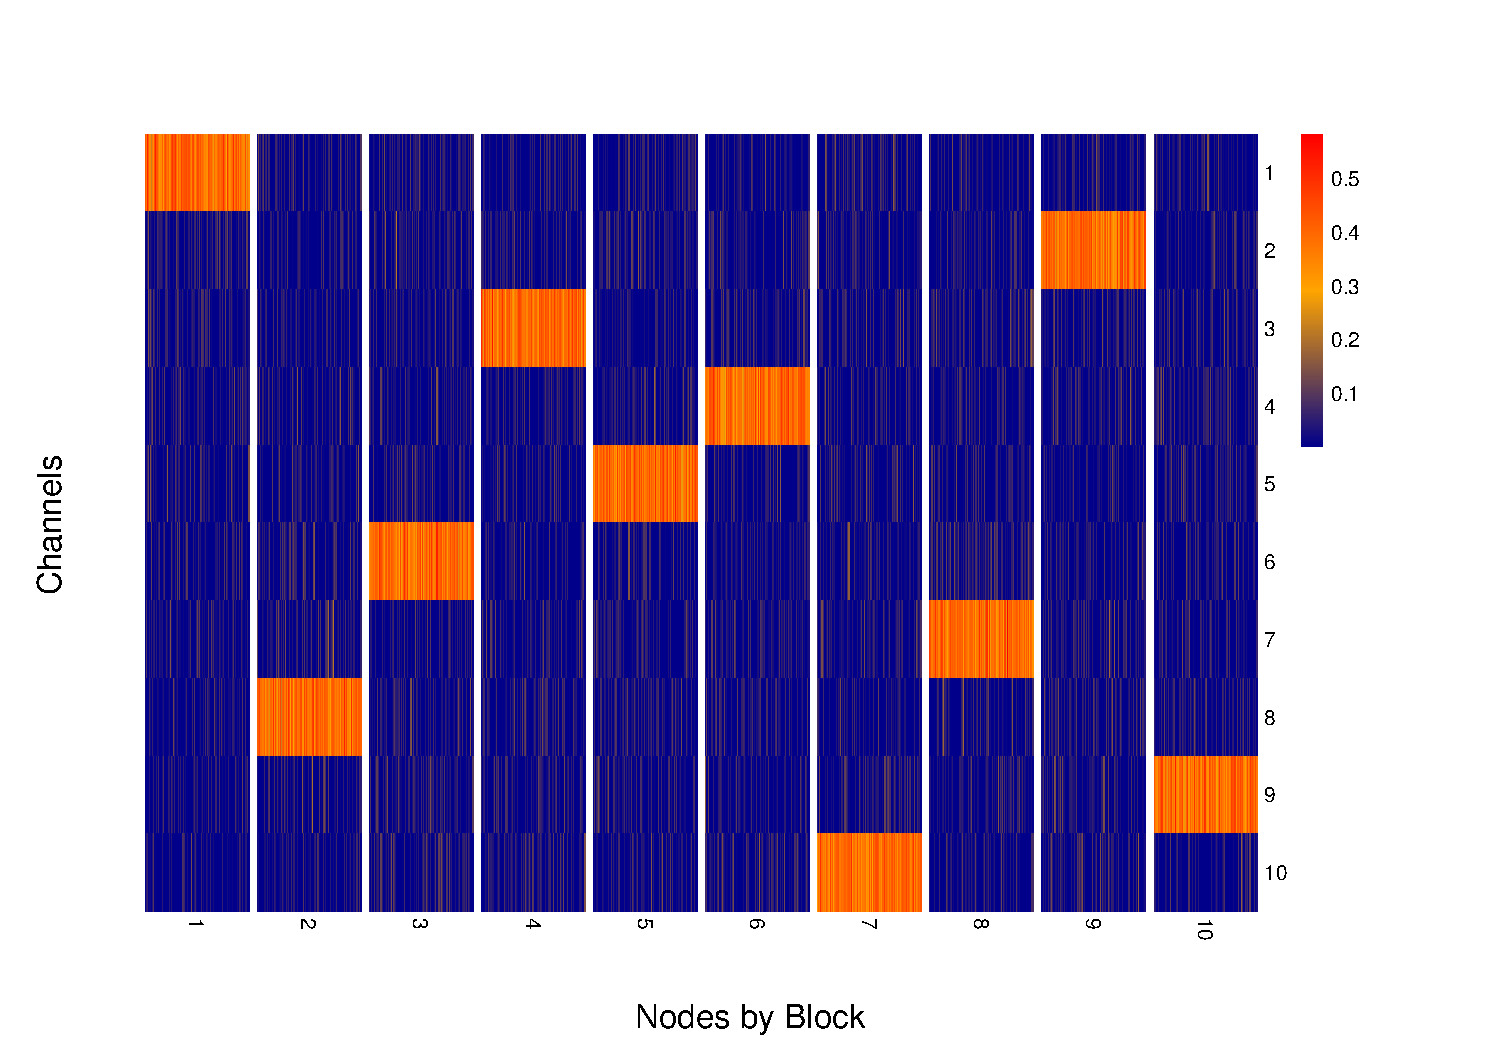
\includegraphics[width = 12cm]{baseSBM.pdf}
\caption{Latent channel model fit to a random stochastic block model. In each block, $p_{in} = 0.25$ and $p_{out} = 0.025$.
Vertical blue lines are used to separate blocks.}
\label{fig:sbm}
\end{figure}

One issue with standard SBMs is their sensitivity to high degree nodes. 
To emulate this, we augmented our original simulated SBM with one hundred new nodes that had an edge probability of 0.25 
to \emph{all} nodes of the graph. We refit the model and plotted on figure \ref{fig:sbmOutliers}. 
We can see that the original structure remains largely intact, 
while the new high degree nodes are strongly attached to all of the latent channels. 

\begin{figure}
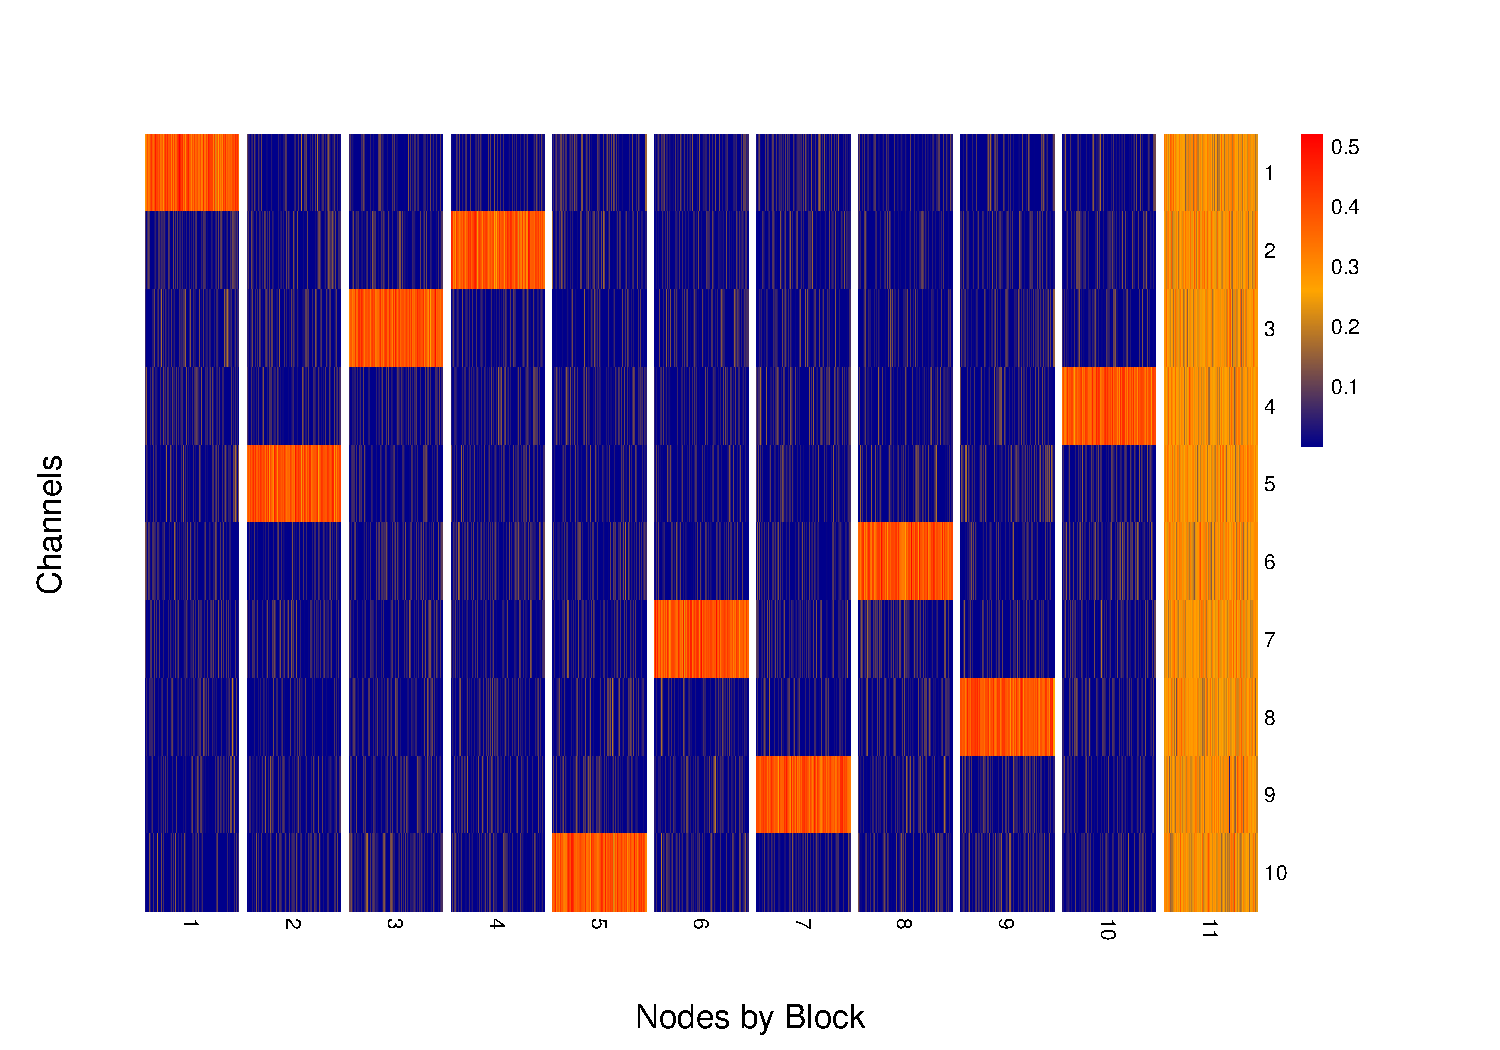
\includegraphics[width = 12cm]{augSBM.pdf}
\caption{Latent channel model fit to a random stochastic block model, augmented with one hundred high degree nodes seen on the far right. 
Vertical blue lines are used to separate blocks.
Note that the overall membership structure remains the same for all the original nodes, but the ten new nodes are strongly attached to every channel.}
\label{fig:sbmOutliers}
\end{figure}

\subsection{email-Eu-core Network}

An email network dataset was built between professors at a university, 
with edges existing if at least one email was sent between the two professors \cite{eu1}, \cite{eu2}. 
The data was downloaded from the Stanford Large Network Dataset Collection \cite{snapnets}.
This network contained 1005 nodes and 24,929 edges (after removing singular loops). In addition, the department 
of each professor was recorded. A total of forty two departments were listed, with department 
size ranging from 109 to 1. A histogram of department size can be found on figure \ref{fig:departSize}.

\begin{figure}
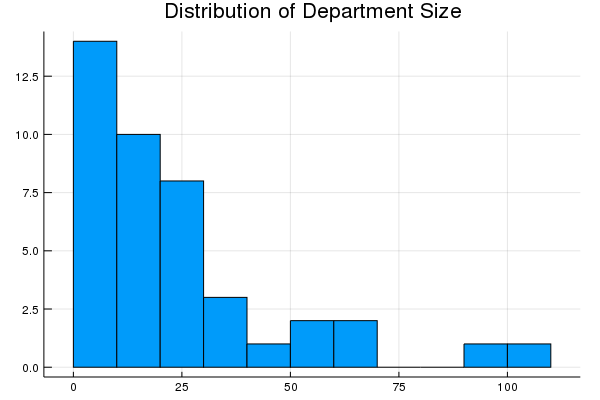
\includegraphics[width = 11cm]{departSize.png}
\caption{Distribution of department size for email-Eu-core network}
\label{fig:departSize}
\end{figure}

We fit four latent channel models to this data with 5, 10, 20 and 40 channels. 
The results can be seen on \ref{fig:emailHubs}. 
Because our model is a maximum likelihood estimator, AIC \cite{aic} can be used 
for model selection. Between our four models, the model with 10 channels has the lowest 
AIC. 

\begin{figure}
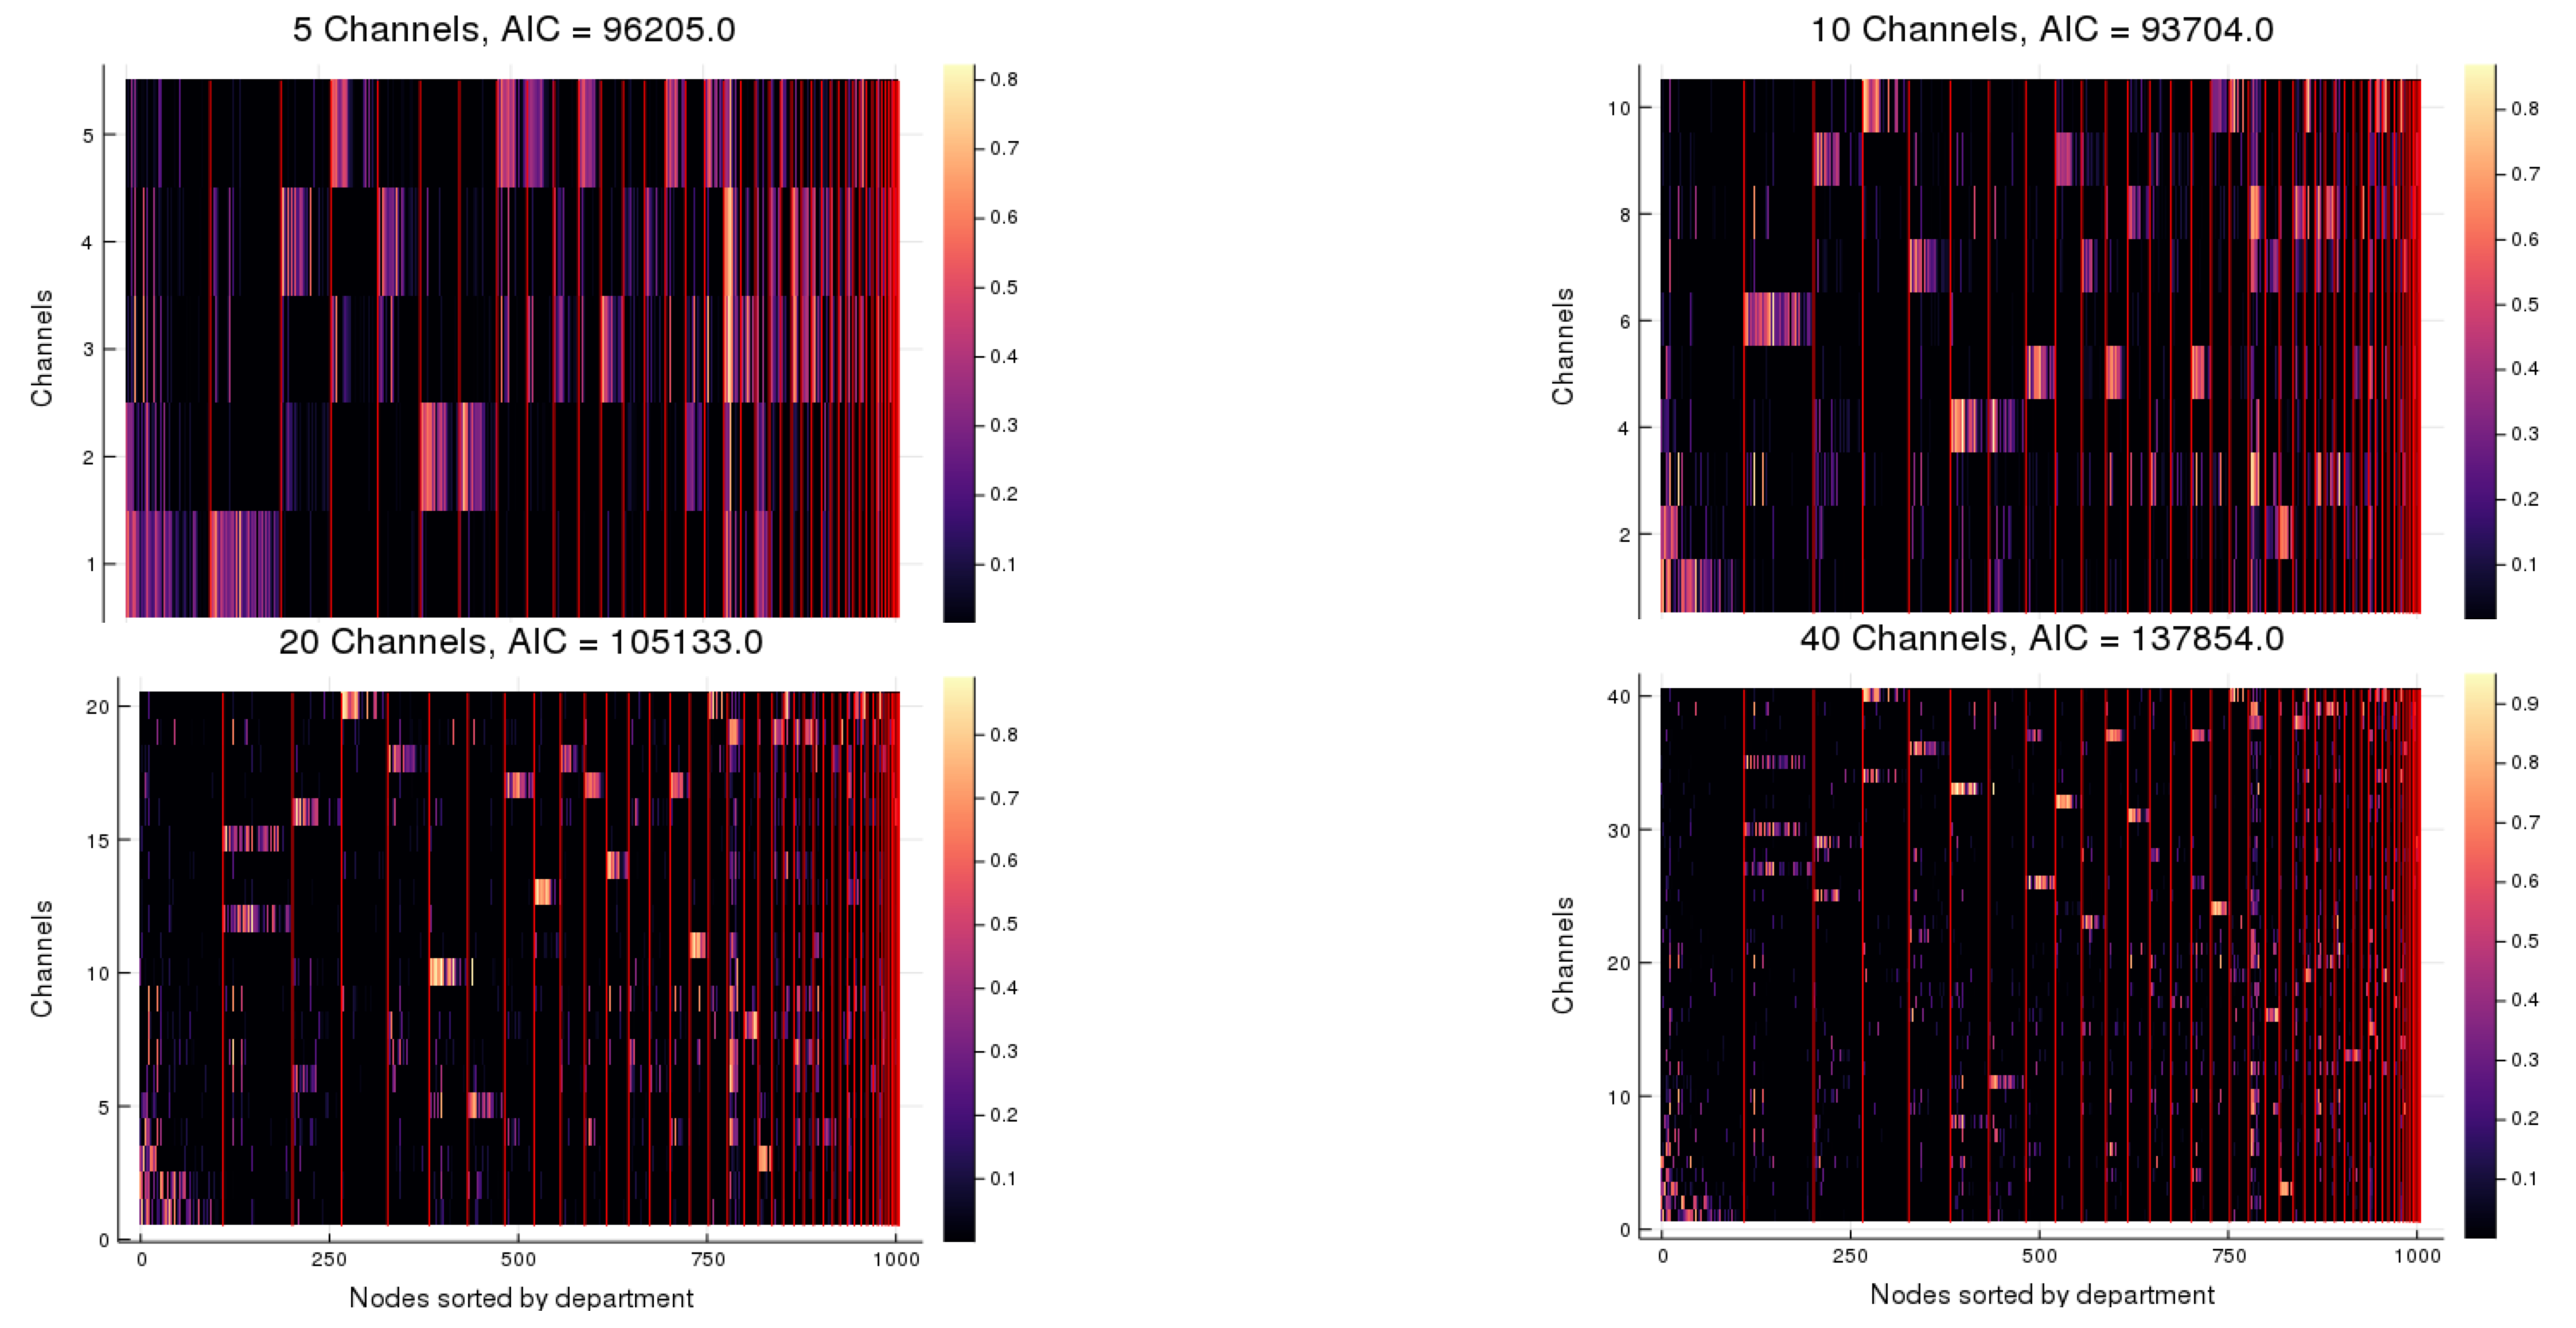
\includegraphics[width = 12cm]{emailChannels.png}
\caption{Email network with 5, 10, 20 and 40 channels. Vertical blue lines are used to separate departments.}
\label{fig:emailHubs}
\end{figure}

We examine the heatmap with 10 channels in more detail in \ref{fig:interestingHub}. 
Within several of the departments, we see that several of the faculty 
are strongly attached to a similar channel. Clearly, not all 42 departments 
are fit to their own channel, but this is not very surprising given the large number of 
very small departments. Of each of the channels, the estimate channel sizes $\hat S_{ik}$
ranged from 39.6 to 62.0. 


\begin{figure}
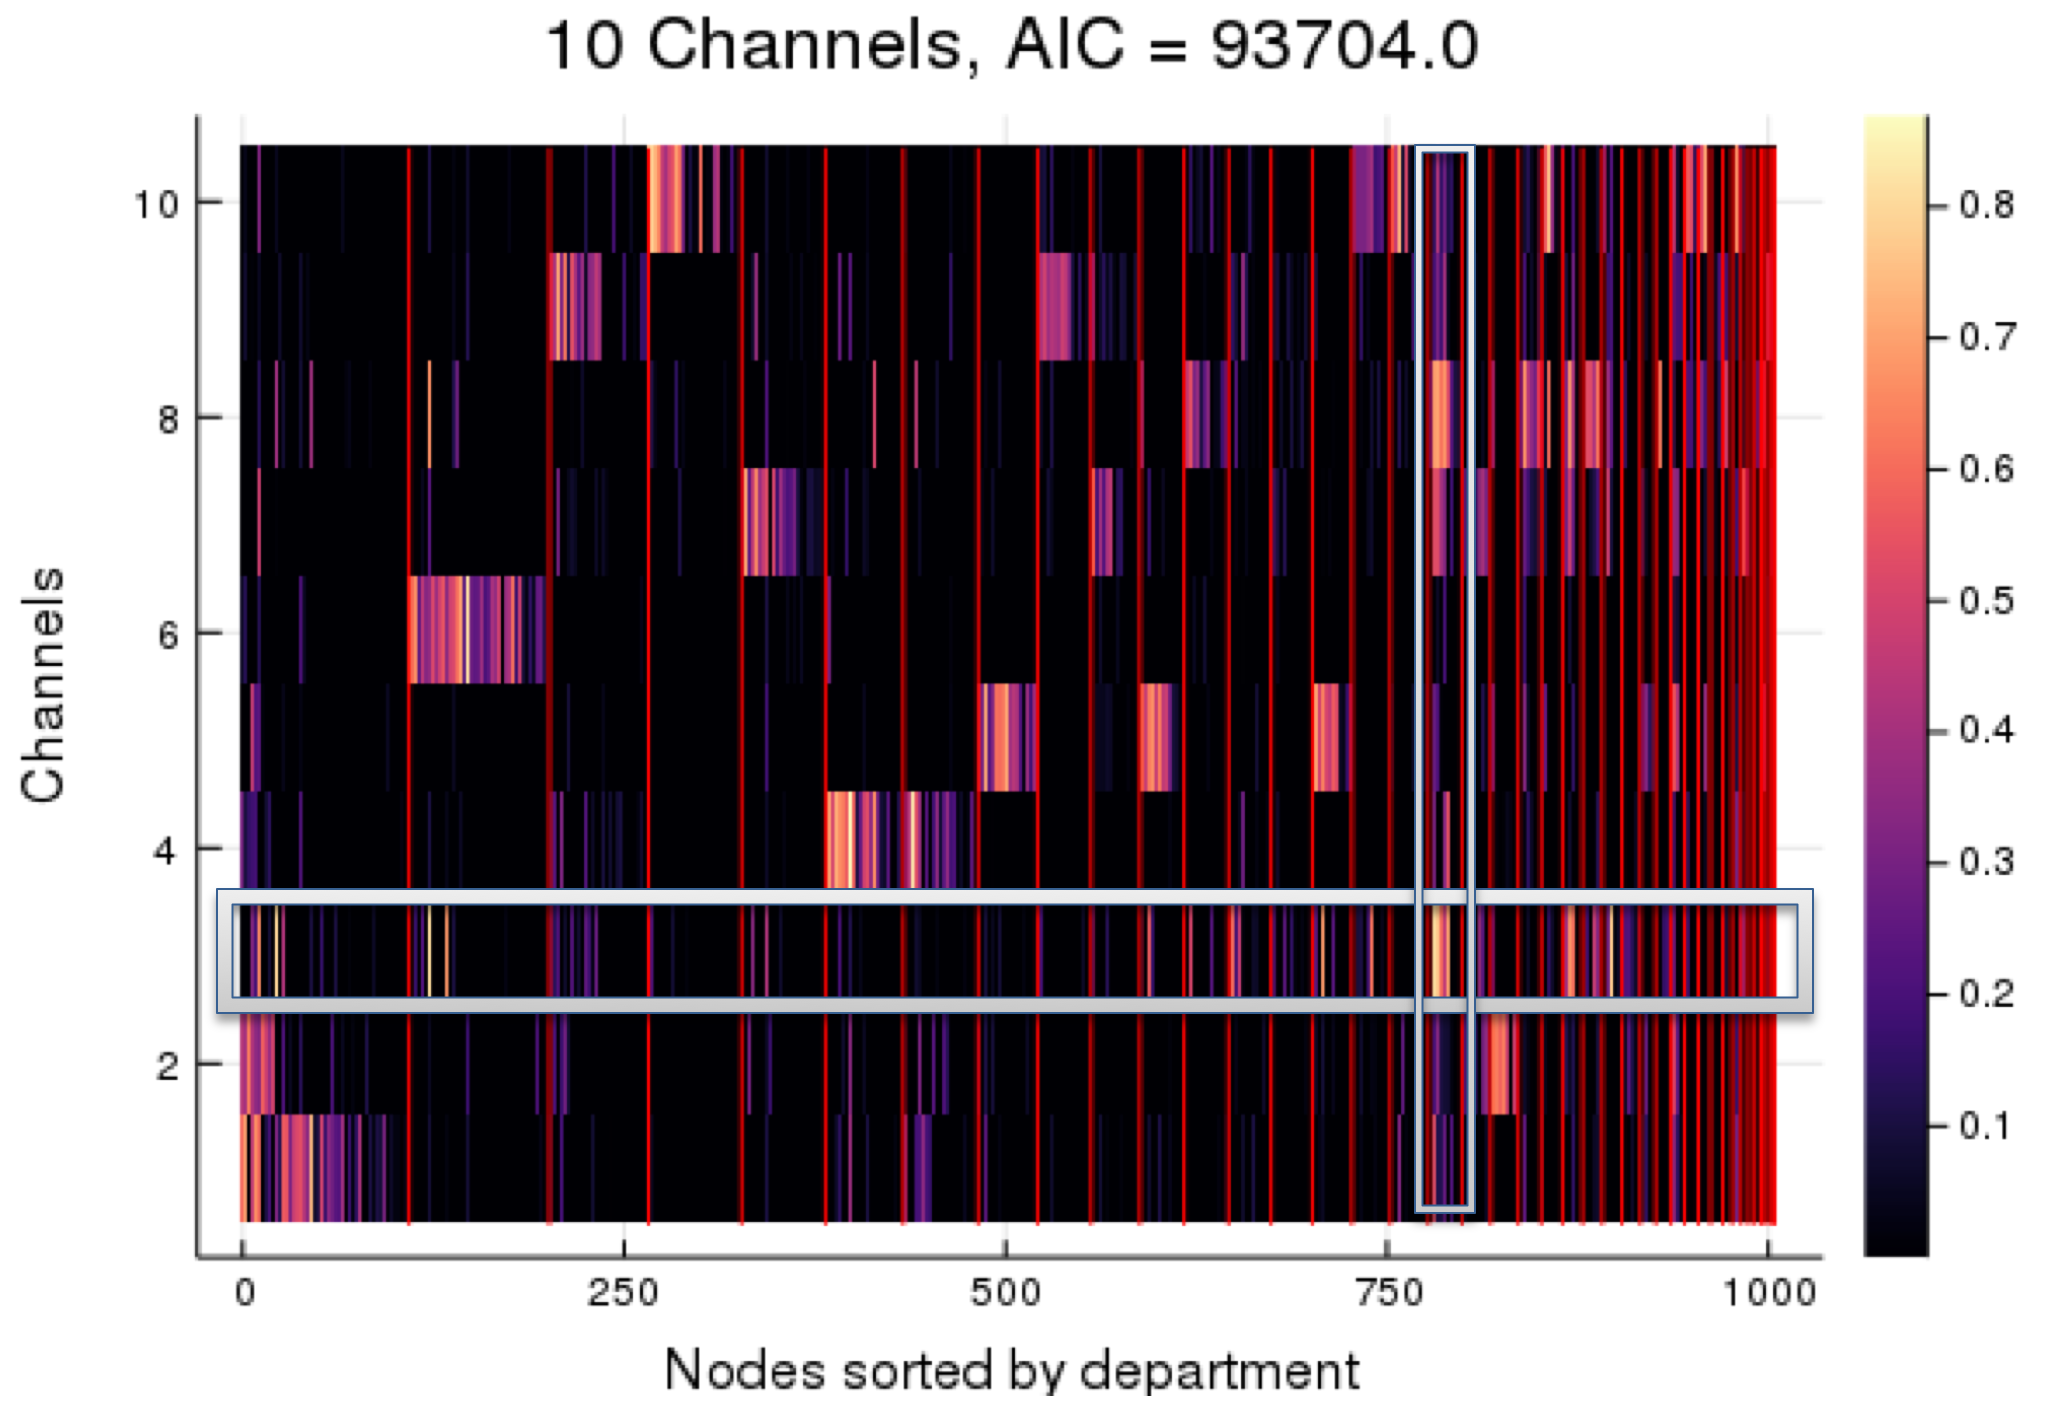
\includegraphics[width = 12cm]{interestingChannel.png}
\caption{Email network with 10 channels.}
\label{fig:interestingHub}
\end{figure}

On figure \ref{fig:interestingHub}, we have highlighted what we consider 
to be a particularly interesting department and channel. 
We see that within this department, several of the nodes are 
attached to \emph{many} channels. In contrast, most other departments 
tend to only have a very few number of nodes strongly attached 
to more than one node. Similarly, there is one channel that is strongly 
attached to this department, which we have highlighted. 
We note that within other departments, 
there tend to be a small number of nodes attached to this channel. 
This suggests that this department communicates with other 
departments in very different ways. 
We hypothesize that this department could actually be an administrative group.

\subsection{Facebook100: UC Berkeley}

Next, we examine the UC Berkeley subset of the Facebook100 graph sets \cite{fb100}. 
The UC-Berkeley graph contains 22,937 nodes with 852,445 edges. 
Several features are collected on each node. 
For this analysis, we consider gender, faculty/student status, 
major and graduation year. 

Rather than selecting the number of channels via AIC

\bibliographystyle{siam}
\bibliography{LatentHubs.bib}

\end{document}  